\documentclass{standalone}
\usepackage{tikz}
\usepackage{ctex,siunitx}
\usepackage{tkz-euclide}
\usepackage{amsmath}
\usetikzlibrary{patterns, calc}
\usetikzlibrary {decorations.pathmorphing, decorations.pathreplacing, decorations.shapes,}
\begin{document}
\small
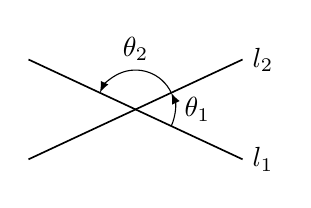
\begin{tikzpicture}[>=latex,scale=1.0]
  \draw[semithick](155:1.5)--(-25:1.5)node[right]{$l_1$};
  \draw[semithick](-155:1.5)--(25:1.5)node[right]{$l_2$};
  \draw[thin,->](-25:0.5)arc(-25:25:0.5)node[midway,right]{$\theta_1$};
  \draw[thin,->](25:0.5)arc(25:155:0.5)node[midway,above]{$\theta_2$};
\end{tikzpicture}
\end{document}